\documentclass{article}
\usepackage[headheight=40pt, textheight=560pt]{geometry}
\usepackage{paralist}
\usepackage{scalerel,amssymb}
\usepackage{amsmath}
\usepackage{colortbl}
\usepackage{array}
\usepackage{multirow}
\usepackage{blindtext}
\usepackage{reledmac}
\usepackage{changepage}

\usepackage{pgfplots}
\usepackage{tikz}
\usetikzlibrary{positioning}
\usetikzlibrary{shapes.geometric, arrows}
\tikzstyle{arrow} = [thick,->,>=stealth]

\usepackage{graphicx}
\usepackage{stix}

\newcommand{\tableflip}{$($\rotatebox{45}{$\smile$}$^{\circ}\smwhtsquare^{\circ})\rotatebox{45}{$\smile$}\mkern-6mu\frown$\raisebox{0.5ex}{$\bot$}$\mkern-3.5mu-\mkern-3.5mu$\raisebox{0.5ex}{$\bot$}}

\usepackage{stackengine}
\def\apeqA{\SavedStyle\sim}
\def\apeq{\setstackgap{L}{\dimexpr.5pt+1.5\LMpt}\ensurestackMath{%
  \ThisStyle{\mathrel{\Centerstack{{\apeqA} {\apeqA} {\apeqA}}}}}}

\usepackage{fancyhdr}
\fancyhead[L]{
	\begin{tabular}{lll}
		\begin{tabular}{l}
			\includegraphics[scale=0.07]{security_lock}
		\end{tabular}	
		&
		\begin{tabular}{l}
			\LARGE \textbf{Cryptography} \\
			\Large \textsc{Zusammenfassung}
		\end{tabular}
		&
		\begin{tabular}{l}
			\tableflip
		\end{tabular}
	\end{tabular}
}
\fancyhead[R]{16-124-836 \\
Marcel \textsc{Zauder}}
\renewcommand{\headrulewidth}{0.4pt}
\fancyfoot[C]{\thepage}
\renewcommand{\footrulewidth}{0.4pt}

\usepackage{hyperref}

\begin{document}
	\pagestyle{fancy}
	\section{One Time Pad}
		\begin{adjustwidth}{2em}{}
			\subsection{What is [\textsc{not}] \textsc{Cryptography}}
			\begin{adjustwidth}{2em}{}
				\subsubsection{Introduction}
					\begin{adjustwidth}{2em}{4em}
						In the idealized model we assume that Alice wants to send a message $m$ (\textit{privately}) to Bob. Alice will modify the message $m$, also called \textit{\textbf{plaintext}}, with any method to create a \textit{\textbf{ciphertext}} $c$ which will be actually sent to Bob. This transformation is also called encryption (\textit{\textbf{Enc}}). After receiving the ciphertext $c$, Bob will reverse the step of transforming by using a decription algorithm (\textit{\textbf{Dec}}) to (\textit{hopefully}) get the original plaintext $m$. \\
						\textit{\textbf{\textsc{Note:}}} We are not trying to hide that a message is sent, so an \textbf{\textsc{Eavesdropper}} (an attacker between Alice and Bob) can obtain the ciphertext $c$ at any instance. Hiding the existence of communication is called \textit{steganography}.
						\\
						\begin{adjustwidth}{1em}{}
							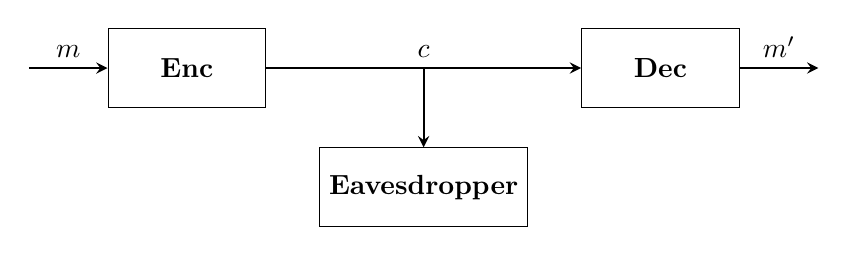
\begin{tikzpicture}
								\coordinate (start);
							
								%Nodes
								\node (rect) [draw,thin,minimum width=2cm,minimum height=1cm, right=of start] (Enc) {\textsc{\textbf{Enc}}};
								\node (rect) [draw,thin,minimum width=2cm,minimum height=1cm, right=4cm of Enc] (Dec) {\textsc{\textbf{Dec}}};
								\node (rect) [draw,thin,minimum width=2cm,minimum height=1cm, below right=0.5cm and 0.675cm of Enc] (Eve) {\textsc{\textbf{Eavesdropper}}};
								\node [right=of Dec] (stop) {};
							
								%Lines
								\draw[arrow] (start) -- node[ anchor=south ]{$m$} (Enc.west);
								\draw[arrow] (Enc.east) -- node[ anchor=south ]{$c$} (Dec.west);
								\draw[arrow] (Enc.east) -| (Eve.north);
								\draw[arrow] (Dec.east) -- node[ anchor=south ]{$m'$} (stop.west);
							
							\end{tikzpicture}
						\end{adjustwidth}
					\end{adjustwidth}
				\subsubsection{Kerckhoff's principle}
				\begin{adjustwidth}{2em}{4em}
					\textit{The method must not be required to be secret, and it must be able to fall into the enemy's hands without causing any inconvenience.} \\ \\
					So if the algorithm do not need to be secret, there must be additional information in the system, which is kept secret from any \textsc{\textbf{Eavesdropper}}. This information is called a \textbf{(secret) key} $k$. 
					\\
					\begin{adjustwidth}{1em}{}
						\begin{tikzpicture}							
							%Nodes
							\node (rect) [draw,thin,minimum width=2cm,minimum height=1cm, right=of start] (KeyGen) {\textsc{\textbf{KeyGen()}}};
							\node [below=of KeyGen] (start) {};
							\node (rect) [draw,thin,minimum width=2cm,minimum height=1cm, right=of start] (Enc) {\textsc{\textbf{Enc}}};
							\node (rect) [draw,thin,minimum width=2cm,minimum height=1cm, below right=0.5cm and 0.675cm of Enc] (Eve) {\textsc{\textbf{Eavesdropper}}};
							\node (rect) [draw,thin,minimum width=2cm,minimum height=1cm, right=4cm of Enc] (Dec) {\textsc{\textbf{Dec}}};
							\node [right=of Dec] (stop) {};
							
							%Lines
							\draw[arrow] (KeyGen.east) -| node[ anchor=south ]{$k$} (Enc.north);
							\draw[arrow] (KeyGen.east) -| node[ anchor=south ]{$k$} (Dec.north);
							\draw[arrow] (start) -- node[ anchor=south ]{$m$} (Enc.west);
							\draw[arrow] (Enc.east) -- node[ anchor=south ]{$c$} (Dec.west);
							\draw[arrow] (Enc.east) -| (Eve.north);
							\draw[arrow] (Dec.east) -- node[ anchor=south ]{$m'$} (stop.west);
							
						\end{tikzpicture}
					\end{adjustwidth}
				\end{adjustwidth}
			\end{adjustwidth}
		\end{adjustwidth}
		\newpage
		\begin{adjustwidth}{2em}{}
			\subsection{Specifics of \textsc{One-Time Pad}}
			\begin{adjustwidth}{2em}{4em}
				A \textit{one-time pad} often uses a secret key in the form of a bit string of length $\lambda$. The plain- and ciphertexts are also $\lambda$bit-strings. \\
				The construction of such an one-time pad looks as follows:
				\\
				\begin{adjustwidth}{2em}{}
					\begin{tabular}{lllll}
						\begin{tabular}{|l|}
							\hline
							\underline{\textsc{KeyGen()}} \\
							\ $k \leftarrow \{ 0,1 \} ^{\lambda}$ \\
							\ \textbf{return} $k$ \\
							\hline
						\end{tabular}
						&
						&
						\begin{tabular}{|l|}
							\hline
							\underline{\textsc{Enc}($k$, $m \in \{ 0,1 \} ^{\lambda}$)} \\
							\ $c := k \oplus m$ \\
							\ \textbf{return} $c$ \\
							\hline
						\end{tabular}
						&
						&
						\begin{tabular}{|l|}
							\hline
							\underline{\textsc{Dec}($k$, $c \in \{ 0,1 \} ^{\lambda}$)} \\
							\ $m' := k \oplus c$ \\
							\ \textbf{return} $m'$ \\
							\hline
						\end{tabular}
					\end{tabular}
				\end{adjustwidth}
				\hfill \\
				Recapture that $k \leftarrow \{ 0,1 \} ^{\lambda}$ means that $k$ is sampled uniformly from the set of $\lambda$bit-strings. \\
				Further we claim that for all $k,m \in \{ 0,1 \} ^{\lambda}$ it is true, that $Dec(k,Enc(k,m)) = m$. \\
				Otherwise the usage of one-time pad would be silly. \\
				For security reasons we want to say about the encryption scheme that an \textsc{Eavesdropper} (who does not know $k$) cannot leran anything about the message $m$. \\
				In the end we need to claim that an encryption algorithm is \textit{secure} if for every $m \in \{ 0,1 \} ^{\lambda}$ the distribution \textsc{Eavesdrop}($m$) is the \textbf{uniform distribution} of $\{ 0,1 \} ^{\lambda}$, explicitly for every $m,m' \in \{ 0,1 \} ^{\lambda}$ the distributions \textsc{Eavesdrop}($m$) and \textsc{Eavesdrop}($m'$) are identical.
			\end{adjustwidth}
		\end{adjustwidth}
		
	\section{The Basics of Proveable Security}
		\begin{adjustwidth}{2em}{}
			\subsection{Generalizing and Abstracting One-Time Pad}
			\begin{adjustwidth}{2em}{}
				\subsubsection{Syntax \& Correctness}
				\begin{adjustwidth}{2em}{4em}
					A \textbf{symmetric key encryption \textit{(SKE)} scheme} consissts of the following algorithms:
					\begin{enumerate}[$\triangleright$]
						\item \textsc{KeyGen}: a randomized algorithm that outputs a \textbf{\textit{key}} $k \in \mathbb{K}$
						\item \textsc{Enc}: a (\textit{possibly randomized}) algorithm that takes a key $k \in \mathbb{K}$ and \textbf{\textit{plaintext}} $m \in \mathbb{M}$ as input, and ouputs a \textbf{\textit{ciphertext}} $c \in \mathbb{C}$
						\item \textsc{Dec}: a deterministic algorithm that takes a key $k \in \mathbb{K}$ and a ciphertexts $c \in \mathbb{C}$ as input, and outputs a plaintext $m \in \mathbb{M}$
					\end{enumerate}
					$\mathbb{K}$ is called the \textbf{\textit{key space}}, $\mathbb{M}$ the \textbf{\textit{message space}}, and $\mathbb{C}$ the \textbf{\textit{ciphertext space}} of the scheme. Often the entire scheme (with all its algorithms) is referred to as $\Sigma$. Each component is then referred to as $\Sigma$.\textsc{KeyGen}, $\Sigma$.\textsc{Enc}, $\Sigma$.\textsc{Dec}, $\Sigma.\mathbb{K}$, $\Sigma.\mathbb{M}$, and $\Sigma.\mathbb{C}$. \\ \\
					Furthermore we define an encryption scheme to be \textbf{\textit{correct}} if for all $k \in \mathbb{K}$ and all $m \in \mathbb{M}$:
					\[
						Pr[\Sigma.\textsc{Dec}(k, \Sigma.\textsc{Enc}(k, m))=m] \ = \ 1 
					\]
					In other words, decrypting a ciphertext, using the same key used for encryption, \textbf{\textit{always}} results in the original plaintext.
				\end{adjustwidth}
			\end{adjustwidth}
			\newpage
			\subsection{Towards an Abstract Security Definition}
			\begin{adjustwidth}{2em}{4em}
				With the properties of one-time pad shown in the first chapter a first attempt can be made to define security: \\
				\textit{For all $m \in \{ 0,1 \}^{\lambda}$, the output of the following subroutine is uniformly distributed over $\{ 0,1 \}^{\lambda}$:}
				\begin{center}
					\begin{tabular}{|l|}
						\hline
						\underline{\textsc{Eavesdrop}($m \in \{ 0,1 \}^{\lambda}$):} \\
						\ \ $k \leftarrow \{ 0,1 \}^{\lambda}$ \\
						\ \ $c \ := \ k \oplus m$ \\
						\ \ \textbf{return} $c$ \\
						\hline
					\end{tabular}
				\end{center}
				\hfill \\
				This property is too specific to one-time pad. To get a more general-purpose security definition, we can write the subroutine using the totally generic encryption scheme $\Sigma$: \\
				\begin{center}
					\begin{tabular}{|l|}
						\hline
						\underline{\textsc{Eavesdrop}($m \in \Sigma.\mathbb{M}$):} \\
						\ \ $k \leftarrow \Sigma.\mathbb{K}$ \\
						\ \ $c \ := \ \Sigma.\textsc{Enc}(k,m)$ \\
						\ \ \textbf{return} $c$ \\
						\hline
					\end{tabular}
				\end{center}
				\hfill \\
				Such an encryption scheme $\Sigma$ is \textit{secure} if, for all $m \in \Sigma.\mathbb{M}$, the output of this subroutine is uniformly distributed over $\Sigma.\mathbb{C}$. 
				\subsubsection{Adversary as Distinguishers}
				\begin{adjustwidth}{2em}{}
					For a better conceptualization of the security definition we consider the following two libraries: \\
					\begin{center}
						\begin{tabular}{lll}
							\begin{tabular}{|l|}
								\hline
								\underline{\textsc{Eavesdrop}($m \in \Sigma.\mathbb{M}$):} \\
								\ \ $k \leftarrow \Sigma.\mathbb{K}$ \\
								\ \ $c \ := \ \Sigma.\textsc{Enc}(k,m)$ \\
								\ \ \textbf{return} $c$ \\
								\hline
							\end{tabular}
							&
							&
							\begin{tabular}{|l|}
								\hline
								\underline{\textsc{Eavesdrop}($m \in \Sigma.\mathbb{M}$):} \\
								\ \ $c \ \leftarrow \ \Sigma.\mathbb{C}$ \\
								\ \ \textbf{return} $c$ \\
								\hline
							\end{tabular}
						\end{tabular}
					\end{center}
					\hfill \\
					$\Sigma$ is \textit{secure} if both implementations of the subroutine \textsc{Eavesdrop} have the same \textit{input-output behavior} (both subroutines generate the same output distribution, on every input). \\
					Furthermore for every calling program $\mathbb{A}$ the connection with the right or left version of the subroutine \textsc{Eavesdrop} should not change the output distribution of $\mathbb{A}$. Such an $\mathbb{A}$ is called an \textit{\textbf{adversary}} which gets too choose plaintexts to send to an \textsc{Eavesdrop} subroutine, but does not know which one of the left or right version is used. Its only goal is to \textbf{distinguish} betwenn the left and right implementation. This means to detect differences in the behavior of the two subroutines. To distinguish whether our implementation is \textit{secure}, the following must hold:
					\[
						Pr[\textit{the adversary outputs \textbf{1} if connected to the left implementation}] $$$$
						= $$$$
						Pr[\textit{the adversary outputs \textbf{1} if connected to the right implementation}]
					\]
					\newpage
					\paragraph{2.2.1.1 Example of a \textit{non-secure} $\Sigma$}
					\begin{adjustwidth}{2em}{}
						In order to add some redundancy to the data, the following OTP is used:
					\end{adjustwidth}
					\begin{adjustwidth}{-1em}{}
						\begin{center}
							\begin{tabular}{|llll|}
								\hline
								\begin{tabular}{l}
									$\mathbb{K} \ = \ \{ 0,1 \}^{\lambda}$ \\
									$\mathbb{M} \ = \ \{ 0,1 \}^{\lambda}$ \\
									$\mathbb{C} \ = \ \{ 0,1 \}^{2\lambda}$ \\
								\end{tabular}
								&
								\begin{tabular}{l}
									\underline{\textsc{KeyGen:}} \\
									\ $k \leftarrow \mathbb{K}$ \\
									\ \textbf{return} $k$
								\end{tabular}
								&
								\begin{tabular}{l}
									\underline{\textsc{Enc}($k, m \in \mathbb{M}$)} \\
									\ $c' \ = \ k \oplus m$ \\
									\ $c \ := \ c' \| c'$ \\
									\ \textbf{return} $c$
								\end{tabular}
								&
								\begin{tabular}{l}
									\underline{\textsc{Dec}($k, c \in \mathbb{C}$)} \\
									\ $c' \ = \ first  \ \lambda \ bits \ of \ c$ \\
									\ \textbf{return} $c' \oplus k$
								\end{tabular}
							\hfill \\
							\hline
							\end{tabular}
						\end{center}
					\end{adjustwidth}
					\hfill \\
					\begin{adjustwidth}{2em}{}
						Intuitively this version of OTP should be also \textit{secure}. However doubling the output ciphertext does not meet the security definition from above. \\
						We can write an adversary which can distinguish between this scheme and a totally random subroutine version:
						\begin{center}
							\begin{tabular}{|l|}
								\hline
								\cellcolor{gray!80} \textsc{Adversary} $\mathbb{A}$ \\
								\ $c \ =$ \textsc{Eavesdrop}($0^{\lambda}$) \\
								\ $L \ =$ first half of $c$ \\
								\ $R \ =$ second half of $c$ \\
								\ \textbf{return} $L \stackrel{?}{=} R$	\\										\hline
							\end{tabular}
						\end{center}
						\hfill \\
						For the doubling version of the subroutine this distinguisher will \textbf{always} return 1. The probability that a fully random subroutine returns a ciphertext with equal first and second halves is $\frac{1}{2^{\lambda}}$. Therefore the probabilities are not equal and the adversary can successfully distinguish between both implementations
					\end{adjustwidth}
				\end{adjustwidth}
				\subsubsection{Chosen Plaintext Attack Template}
				\begin{adjustwidth}{2em}{}
					In general the "doubling-OTP" is \textit{secure} over the distributione of $2\lambda$-bit-strings with the same first and second half. We required \textsc{Eavesdrop} to be uniform, while the more useful definition is that \textsc{Eavesdrop} is uniform for all $m$. Therefore we got another approach for the security definition: \\
					$\Sigma$ is \textit{secure} if, for all calling programs $\mathbb{A}$, the distribution of the following two subroutines does not differ: \\
					\begin{center}
						\begin{tabular}{lll}
							\begin{tabular}{|l|}
								\hline
								\underline{\textsc{Eavesdrop}($m_L , m_R \in \Sigma.\mathbb{M}$):} \\
								\ \ $k \leftarrow \Sigma.\mathbb{K}$ \\
								\ \ $c \ := \ \Sigma.\textsc{Enc}(k,m_L)$ \\
								\ \ \textbf{return} $c$ \\
								\hline
							\end{tabular}
							&
							&
							\begin{tabular}{|l|}
								\hline
								\underline{\textsc{Eavesdrop}($m_L , m_R \in \Sigma.\mathbb{M}$):} \\
								\ \ $k \leftarrow \Sigma.\mathbb{K}$ \\
								\ \ $c \ := \ \Sigma.\textsc{Enc}(k,m_R)$ \\
								\ \ \textbf{return} $c$ \\
								\hline
							\end{tabular}
						\end{tabular}
					\end{center}
					\hfill \\
					A calling program chooses two (different) plaintexts and give them to the subroutine. Each \textsc{Eavesdrop} ignores one of the inputs and only encrypts one plaintext. If this subroutine is \textit{secure} an adversary cannot distinguish between the two implementations because they will have the same input/output behavior. Otherwise $\mathbb{A}$ can see a difference which contriutes against the security definition. \\
					These sort of "attacks" are called \textbf{chosen-plaintext} attacks. This security definition is based on that you cannot get any information from the ciphertext about the plaintext - even if you know it was only one of two options - which you have chosen.
				\end{adjustwidth}
			\end{adjustwidth}
			\subsection{Provable Security Fundamentals}
			\begin{adjustwidth}{2em}{}
				\subsubsection{Libraries \& Interfaces}
				\begin{adjustwidth}{2em}{4em}
					A \textbf{\textit{library}} $\mathbb{L}$ is a collection of subroutines and \textit{private/static} variables. A library is often represented in its \textbf{\textit{interface}} form, in which the names, argument types and, output types of all its subroutines are stated. \\
					When a calling program $\mathbb{A}$ is linked to a distinct library we write: $\mathbb{A} \diamond \mathbb{L}$, which means that the implementation of a subroutine stated in the library $\mathbb{L}$ is used. The event that $\mathbb{A} \diamond \mathbb{L}$ outputs the value $z$ is written as $\mathbb{A} \diamond \mathbb{L} \Rightarrow z$.
					\paragraph{2.3.1.1 Example for linking adversary and interfaces}
					\begin{adjustwidth}{2em}{}
						We consider the following libraries $\mathbb{L}_1$ and $\mathbb{L}_2$ (which we have seen before): \\
						\begin{center}
							\begin{tabular}{lll}
								\begin{tabular}{|l|}
									\hline
									\cellcolor{gray!80} \textbf{\textit{Library}} $\mathbb{L}_1$ \\
									\hline
									\underline{\textsc{Eavesdrop}(m):} \\
									\ \ $k \leftarrow \{ 0,1 \}^{\lambda}$ \\
									\ \ $c' := k \oplus m$ \\
									\ \ \textbf{return} $c' \| c'$ \\
									\hline
								\end{tabular}
								&
								&
								\begin{tabular}{|l|}
									\hline
									\cellcolor{gray!80} \textbf{\textit{Library}} $\mathbb{L}_2$ \\
									\hline
									\underline{\textsc{Eavesdrop}(m):} \\
									\ \ $c \leftarrow \{ 0,1 \}^{2\lambda}$ \\
									\ \ \textbf{return} $c$ \\
									\hline
								\end{tabular}
							\end{tabular}
						\end{center}
						\hfill \\
						And the following adversary $\mathbb{A}$: \\
						\begin{center}
							\begin{tabular}{|l|}
								\hline
								\cellcolor{gray!80} \textbf{\textit{Adversary}} $\mathbb{A}$ \\
								\hline
								$c := \ \textsc{Eavesdrop}(0^{\lambda})$ \\
								$L :=$ first half of $c$ \\
								$R :=$ second half of $c$ \\
								\textbf{return} $L \stackrel{?}{=} R$ \\
								\hline							
							\end{tabular}
						\end{center}
						\hfill \\
						The outputs of the previously discussed form are then:
						\begin{align*}
							Pr[\mathbb{A} \diamond \mathbb{L}_1 \Rightarrow \textsc{True}] \ & = \ 1 \\
							Pr[\mathbb{A} \diamond \mathbb{L}_2 \Rightarrow \textsc{True}] \ & = \ \frac{1}{2^{\lambda}}
						\end{align*}						
					\end{adjustwidth}
					\paragraph{2.3.1.2 Example of library interfaces}
					\begin{adjustwidth}{2em}{}
						A library can also contain couple of subroutines: \\
						\begin{center}
							\begin{tabular}{|l|}
								\hline
								\cellcolor{gray!80} \textbf{\textit{Library}} $\mathbb{L}$ \\
								\hline
								$s \leftarrow \{ 0,1 \}^{\lambda}$ \\
								\\
								\underline{\textsc{Reset}():} \\
								\ \ $s \leftarrow \{ 0,1 \}^{\lambda}$ \\
								\\
								\underline{\textsc{Guess}($x \in \{ 0,1 \}^{\lambda}$)} \\
								\ \ \textbf{return} $x \stackrel{?}{=} s$ \\
								\hline							
							\end{tabular}
						\end{center}
						\hfill \\
						Code outside of a subroutine is run one in the initialization. Variables defined in this initialization time (as $s$ in this library) are visible in all subroutine scopes.
					\end{adjustwidth}
				\end{adjustwidth}
				\subsubsection{Interchangeability}
				\begin{adjustwidth}{2em}{4em}
					We call two libraries $\mathbb{L}_{left}$ and $\mathbb{L}_{right}$ \textbf{interchangeable} and write $\mathbb{L}_{left} \equiv \mathbb{L}_{right}$, if for all calling pragrams $\mathbb{A}$ that output a single bit:
					\[
						Pr[\mathbb{A} \diamond \mathbb{L}_{left} \Rightarrow 1] \ = \ Pr[\mathbb{A} \diamond \mathbb{L}_{right} \Rightarrow 1]
					\]
					The interchangeability of libraries includes:
					\begin{adjustwidth}{1em}{}
						\begin{enumerate}[-]
							\item Their only difference happens in an \textit{unreachable block of code}
							\item Their only difference is the value they assign to a \textit{variable that is never actually used}
							\item Their only difference is that one library \textit{unrolls a loop} that occurs in the other library
							\item Their only difference is that one library \textit{inlines a subroutine} that occurs in the other library
						\end{enumerate}
					\end{adjustwidth}
				\end{adjustwidth}
				\subsubsection{Security Definition, Using New Terminology}
				\begin{adjustwidth}{2em}{}
					We say that $\Sigma$ has \textbf{one-time uniform ciphertexts} if $\mathbb{L}^{\Sigma}_{ots\$-real} \equiv \mathbb{L}^{\Sigma}_{ots\$-rand}$, where: \\
					\begin{center}
						\begin{tabular}{lll}
							\begin{tabular}{|l|}
								\hline
								\cellcolor{gray!80} Library $\mathbb{L}^{\Sigma}_{ots\$-real}$ \\
								\hline
								\underline{\textsc{CTxt}($m \in \Sigma.\mathbb{M}$):} \\
								\ \ $k \leftarrow \Sigma.$\textsc{KeyGen} \\
								\ \ $c \leftarrow \Sigma.$\textsc{Enc}($k,m$) \\
								\ \ \textbf{return} $c$ \\
								\hline
							\end{tabular}
							&
							&
							\begin{tabular}{|l|}
								\hline
								\cellcolor{gray!80} Library $\mathbb{L}^{\Sigma}_{ots\$-rand}$ \\
								\hline
								\underline{\textsc{CTxt}($m \in \Sigma.\mathbb{M}$):} \\
								\ \ $c \leftarrow \Sigma.\mathbb{C}$ \\
								\ \ \textbf{return} $c$ \\
								\hline
							\end{tabular}
						\end{tabular}
					\end{center}
					\hfill \\
					We say that $\Sigma$ has \textbf{one-time secrecy} if $\mathbb{L}^{\Sigma}_{ots-R} \equiv \mathbb{L}^{\Sigma}_{ots-L}$, where: \\
					\begin{center}
						\begin{tabular}{lll}
							\begin{tabular}{|l|}
								\hline
								\cellcolor{gray!80} Library $\mathbb{L}^{\Sigma}_{ots-R}$ \\
								\hline
								\underline{\textsc{Eavesdrop}($m_R,m_L \in \Sigma.\mathbb{M}$):} \\
								\ \ $k \leftarrow \Sigma.$\textsc{KeyGen} \\
								\ \ $c \leftarrow \Sigma.$\textsc{Enc}($k, m_R$) \\
								\ \ \textbf{return} $c$ \\
								\hline
							\end{tabular}
							&
							&
							\begin{tabular}{|l|}
								\hline
								\cellcolor{gray!80} Library $\mathbb{L}^{\Sigma}_{ots-L}$ \\
								\hline
								\underline{\textsc{Eavesdrop}($m_R,m_L \in \Sigma.\mathbb{M}$):} \\
								\ \ $k \leftarrow \Sigma.$\textsc{KeyGen} \\
								\ \ $c \leftarrow \Sigma.$\textsc{Enc}($k, m_L$) \\
								\ \ \textbf{return} $c$ \\
								\hline
							\end{tabular}
						\end{tabular}
					\end{center}
				\end{adjustwidth}
			\end{adjustwidth}
			\subsection{How to Prove Security with the Hybrid Technique}
			\begin{adjustwidth}{2em}{}
				\subsubsection{Chaining Several Components}
				\begin{adjustwidth}{2em}{4em}
					If an adversary $\mathbb{A}$ is linked to more than one libraries (for example: $\mathbb{A} \diamond \mathbb{L}_1 \diamond \mathbb{L}_2$) there are several possible ways to interpret this:
					\begin{adjustwidth}{1em}{}
						\begin{enumerate}[-]
							\item $(\mathbb{A} \diamond \mathbb{L}_1) \diamond \mathbb{L}_2$: \\
							A \textbf{compound calling program} linked to $\mathbb{L}_2$. After all, $\mathbb{A} \diamond \mathbb{L}_1$ is a program which calls subroutines of $\mathbb{L}_2$.
							\item $\mathbb{A} \diamond (\mathbb{L}_1 \diamond \mathbb{L}_2)$: \\
							$\mathbb{A}$ is linked to a \textbf{compound library}. After all, $\mathbb{A}$ is a program which calls subroutines of $\mathbb{L}_1 \diamond \mathbb{L}_2$.
						\end{enumerate}
					\end{adjustwidth}
					Note that the placement of the parantheses does \textbf{\textsc{not}} affect the overall program, which will behave the same way in both options.
				\end{adjustwidth}
				\subsubsection{One-Time Secrecy of One-Time Pad}
				\begin{adjustwidth}{2em}{4em}
					For any encryption scheme $\Sigma$ which fulfills the characteristics of \textit{one-time uniform ciphertexts} it holds that it also has \textit{one-time secrecy}, also written as:
					\[
						\mathbb{L}_{ots\$-real}^{\Sigma} \ \equiv \ \mathbb{L}_{ots\$-rand}^{\Sigma} \  \Rightarrow \ \mathbb{L}_{ots-L}^{\Sigma} \ \equiv \ \mathbb{L}_{ots-R}^{\Sigma}
					\]
					We will prove this by using the \textbf{\textit{hybrid technique}}: \\
					The scheme for this type of prove is the following:
					\[
						\mathbb{L}_{ots-L}^{\Sigma} \ \equiv \ \mathbb{L}_{hyb-1} \ \equiv \ \mathbb{L}_{hyb-2} \ \equiv \ \mathbb{L}_{hyb-3} \ \equiv \ \ldots \ \equiv \ \mathbb{L}_{ots-R}^{\Sigma}
					\]
					where $\mathbb{L}_{hyb-1}, \ \mathbb{L}_{hyb-2}, \ldots$ are so called \textbf{\textit{hybrid}} libraries, which can be chosen nearly randomly.
					For this prove we will use that $\mathbb{L}_{ots\$-real}^{\Sigma} \ \equiv \ \mathbb{L}_{ots\$-rand}^{\Sigma}$ holds and show that $\mathbb{L}_{ots-L}^{\Sigma} \ \equiv \ \mathbb{L}_{ots-R}^{\Sigma}$ also holds:
				\end{adjustwidth}
				\begin{adjustwidth}{-6em}{}
					\begin{center}
						\begin{tabular}{lllll}
							\begin{tabular}{c}
								$\mathbb{L}_{ots-L}^{\Sigma}$:
							\end{tabular}
							&
							\begin{tabular}{|l|}
								\hline
								\cellcolor{gray!80} Library $\mathbb{L}^{\Sigma}_{ots-L}$ \\
								\hline
								\underline{\textsc{Eavesdrop}($m_R,m_L \in \Sigma.\mathbb{M}$):} \\
								\ \ $k \leftarrow \Sigma.$\textsc{KeyGen} \\
								\ \ $c \leftarrow \Sigma.$\textsc{Enc}($k, m_L$) \\
								\ \ \textbf{return} $c$ \\
								\hline
							\end{tabular}
							&
							&
							&
							\begin{tabular}{l}
								We start with the library $\mathbb{L}_{ots-L}^{\Sigma}$.
							\end{tabular}
							\\
							\begin{tabular}{c}
								$\mathbb{L}_{hyb-1}$:
							\end{tabular}
							&
							\begin{tabular}{|l|}
								\hline
								\underline{\textsc{Eavesdrop}($m_R,m_L \in \Sigma.\mathbb{M}$):} \\
								\ \ $c \ := \ $ \textsc{CTxt}($m_L$) \\
								\ \ \textbf{return} $c$ \\
								\hline
							\end{tabular}
							&
							\begin{tabular}{l}
								$\diamond$
							\end{tabular}
							&
							\begin{tabular}{|l|}
								\hline
								\cellcolor{gray!80} Library $\mathbb{L}^{\Sigma}_{ots\$-real}$ \\
								\hline
								\underline{\textsc{CTxt}($m \in \Sigma.\mathbb{M}$):} \\
								\ \ $k \leftarrow \Sigma.$\textsc{KeyGen} \\
								\ \ $c \leftarrow \Sigma.$\textsc{Enc}($k,m$) \\
								\ \ \textbf{return} $c$ \\
								\hline
							\end{tabular}
							&
							\begin{tabular}{p{4.5cm}}
								By factoring out the subroutine we do not change the external behaviour of this library. Also we can see that this new subroutine is equal to $\mathbb{L}^{\Sigma}_{ots\$-real}$ we have seen before. 
							\end{tabular}
							\\
							\begin{tabular}{c}
								$\mathbb{L}_{hyb-2}$:
							\end{tabular}
							&
							\begin{tabular}{|l|}
								\hline
								\underline{\textsc{Eavesdrop}($m_R,m_L \in \Sigma.\mathbb{M}$):} \\
								\ \ $c \ := \ $ \textsc{CTxt}($m_L$) \\
								\ \ \textbf{return} $c$ \\
								\hline
							\end{tabular}
							&
							\begin{tabular}{l}
								$\diamond$
							\end{tabular}
							&
							\begin{tabular}{|l|}
								\hline
								\cellcolor{gray!80} Library $\mathbb{L}^{\Sigma}_{ots\$-rand}$ \\
								\hline
								\underline{\textsc{CTxt}($m \in \Sigma.\mathbb{M}$):} \\
								\ \ $c \leftarrow \Sigma.\mathbb{C}$ \\
								\ \ \textbf{return} $c$ \\
								\hline
							\end{tabular}
							&
							\begin{tabular}{p{4.5cm}}
								Because of the previously seen \textit{chaining Lemma} we can change between $\mathbb{L}^{\Sigma}_{ots\$-real}$ and $\mathbb{L}^{\Sigma}_{ots\$-rand}$ which has no effect on its external behaviour (as shown before).
							\end{tabular}
							\\
							\begin{tabular}{c}
								$\mathbb{L}_{hyb-3}$:
							\end{tabular}
							&
							\begin{tabular}{|l|}
								\hline
								\underline{\textsc{Eavesdrop}($m_R,m_L \in \Sigma.\mathbb{M}$):} \\
								\ \ $c \ := \ $ \textsc{CTxt}($m_R$) \\
								\ \ \textbf{return} $c$ \\
								\hline
							\end{tabular}
							&
							\begin{tabular}{l}
								$\diamond$
							\end{tabular}
							&
							\begin{tabular}{|l|}
								\hline
								\cellcolor{gray!80} Library $\mathbb{L}^{\Sigma}_{ots\$-rand}$ \\
								\hline
								\underline{\textsc{CTxt}($m \in \Sigma.\mathbb{M}$):} \\
								\ \ $c \leftarrow \Sigma.\mathbb{C}$ \\
								\ \ \textbf{return} $c$ \\
								\hline
							\end{tabular}
							&
							\begin{tabular}{p{4.5cm}}
								Because \textsc{Ctxt} does not depend on the given argument we can change it from $m_L$ to $m_R$ without any effects to its behaviour.
							\end{tabular}
							\\
							\begin{tabular}{c}
								$\mathbb{L}_{hyb-4}$:
							\end{tabular}
							&
							\begin{tabular}{|l|}
								\hline
								\underline{\textsc{Eavesdrop}($m_R,m_L \in \Sigma.\mathbb{M}$):} \\
								\ \ $c \ := \ $ \textsc{CTxt}($m_R$) \\
								\ \ \textbf{return} $c$ \\
								\hline
							\end{tabular}
							&
							\begin{tabular}{l}
								$\diamond$
							\end{tabular}
							&
							\begin{tabular}{|l|}
								\hline
								\cellcolor{gray!80} Library $\mathbb{L}^{\Sigma}_{ots\$-real}$ \\
								\hline
								\underline{\textsc{CTxt}($m \in \Sigma.\mathbb{M}$):} \\
								\ \ $k \leftarrow \Sigma.$\textsc{KeyGen} \\
								\ \ $c \leftarrow \Sigma.$\textsc{Enc}($k,m$) \\
								\ \ \textbf{return} $c$ \\
								\hline
							\end{tabular}
							&
							\begin{tabular}{p{4.5cm}}
								We reverse the step where we changed the subroutine from $\mathbb{L}^{\Sigma}_{ots\$-real}$ to $\mathbb{L}^{\Sigma}_{ots\$-rand}$.
							\end{tabular}
							\\
							\begin{tabular}{c}
								$\mathbb{L}_{ots-R}^{\Sigma}$:
							\end{tabular}
							&
							\begin{tabular}{|l|}
								\hline
								\cellcolor{gray!80} Library $\mathbb{L}^{\Sigma}_{ots-R}$ \\
								\hline
								\underline{\textsc{Eavesdrop}($m_R,m_L \in \Sigma.\mathbb{M}$):} \\
								\ \ $k \leftarrow \Sigma.$\textsc{KeyGen} \\
								\ \ $c \leftarrow \Sigma.$\textsc{Enc}($k, m_R$) \\
								\ \ \textbf{return} $c$ \\
								\hline
							\end{tabular}
							&
							&
							&
							\begin{tabular}{p{4.5cm}}
								In the end we inline the subroutine and end with the library $\mathbb{L}^{\Sigma}_{ots-R}$. \\
							\end{tabular}
						\end{tabular}
					\end{center}
				\end{adjustwidth}
			\end{adjustwidth}
			\subsection{How to Demonstrate Insecurity with Attacks}
			\begin{adjustwidth}{2em}{4em}
				We will consider the following libraries (left and right version): \\
				\begin{center}
					\begin{tabular}{lll}
						\begin{tabular}{|l|}
							\hline
							\cellcolor{gray!80} Library $\mathbb{L}^{\Sigma}_{ots-L}$ \\
							\hline
							\underline{\textsc{Eavesdrop}($m_R,m_L$):} \\
							\ \ $k \ \leftarrow \ \{ \textit{permutations of } \{ 1, \lambda \} \}$ \\
							\ \ for $i := 1$ to $\lambda$ \\
							\ \ \ \ $c_{k(i)} \ := \ (m_L)_i$ \\
							\ \ \textbf{return} $c_1\ldots c_{\lambda}$ \\
							\hline
						\end{tabular}
						&
						&
						\begin{tabular}{|l|}
							\hline
							\cellcolor{gray!80} Library $\mathbb{L}^{\Sigma}_{ots-R}$ \\
							\hline
							\underline{\textsc{Eavesdrop}($m_R,m_L$):} \\
							\ \ $k \ \leftarrow \ \{ \textit{permutations of } \{ 1, \lambda \} \}$ \\
							\ \ for $i := 1$ to $\lambda$ \\
							\ \ \ \ $c_{k(i)} \ := \ (m_R)_i$ \\
							\ \ \textbf{return} $c_1\ldots c_{\lambda}$ \\
							\hline
						\end{tabular}
					\end{tabular}
				\end{center}
				\hfill \\
				We define the following distinguisher: \\
				\begin{center}
					\begin{tabular}{|l|}
						\hline
						\cellcolor{gray!80} Adversary $\mathbb{A}$ \\
						\hline
						\ \ $c \ \leftarrow$ \textsc{Eavesdrop}($0^{\lambda}$, $1^{\lambda}$) \\
						\ \ \textbf{return} $0^{\lambda} \stackrel{?}{=} c$ \\
						\hline
					\end{tabular}
				\end{center}
				\hfill \\
				Linking $\mathbb{A}$ with either the \textit{left} or \textit{right} version of the library will result in a different behaviour:
				\begin{adjustwidth}{2em}{}
					\begin{enumerate}[]
						\item \underline{$\mathbb{A} \diamond \mathbb{L^{\Sigma}_{ots-L}}$} \\
						\begin{adjustwidth}{2em}{}
							Linking $\mathbb{A}$ with the \textit{left} library will return a $c$ with each bit equal to $0$. Therefore \\ 
							$Pr[\mathbb{A} \diamond \mathbb{L^{\Sigma}_{ots-L}} \Rightarrow 1] \ = \ 1$.
						\end{adjustwidth}
						\item \underline{$\mathbb{A} \diamond \mathbb{L^{\Sigma}_{ots-R}}$} \\
						\begin{adjustwidth}{2em}{}
							Linking $\mathbb{A}$ with the \textit{right} library will return a $c$ with each bit equal to $1$. Therefore \\ 
							$Pr[\mathbb{A} \diamond \mathbb{L^{\Sigma}_{ots-R}} \Rightarrow 1] \ = \ 0$.
						\end{adjustwidth}
					\end{enumerate}
				\end{adjustwidth}
				Therefore the probabilities are different which leads to the conclusion that $\mathbb{A}$ can distinguish between the \textit{left} and \textit{right} library.
			\end{adjustwidth}
		\end{adjustwidth}
	\newpage
	\section{Basing Cryptography on Intractable Computations}
		\begin{adjustwidth}{2em}{}
		\subsection{What Qualifies as a "Computational Infeasible" Attack?}
			\begin{adjustwidth}{2em}{4em}
				\textit{One-time pad} cannot be broken, not even with a \textbf{brute-force} attack, trying all posible keys. However, all schemes that are coming next can be broken by such an attack. To make this more difficult for an \textit{adversary} we use the $\lambda$ parameter that we also call \textbf{security parameter} and choose it large enough to make the attack \textit{impractical}. Ideally every attack (not just a \textbf{brute-force} attack) will have the difficulty roughly $2^{\lambda}$.
				\subsubsection{Asymptotic Running Time}
					\begin{adjustwidth}{2em}{}
						We will now defy where to draw a line between a "\textit{feasible}" attack (which we want to protect against) and an "\textit{infeasible}" one (which we do not need to care about). \\
						We will consider the \textbf{asymptotic} cost of an attack. An algorithm which has a polynomial computation time scale reasonably well (especially if our security parameter is small) whereas one with exponential time do not. We also call a polynomial-time algorithm an "\textit{efficient}" one. \\
						Furthermore with the following \textbf{closure property} the consideration of polynomial-time algorithms is extremely useful: \textit{repeating a polynomial-time algorithm a polynomial number of times result in a polynomial-time proces overall}.
					\end{adjustwidth}
				\subsubsection{Potential Pitfall: Numerical Algorithms}
					\begin{adjustwidth}{2em}{}
						Because we will later discuss algorithms that operate over large numbers (e.g. thousand of bits long) we have to remember that representing this large number $N$ on a computer only requires $\sim log_2 N$ bits. Therefore our security parameter will be $log_2 N$ instead of $N$ which is a huge difference in the ranges of large $N$. \\
						For reference, following are some numerical operations that will be used later: \\ \\
						\begin{tabular}{ccc}
							\begin{tabular}{|l|}
								\hline
								\textbf{Efficient algorithm known:} \\
								\hline
								Computing GCDs \\
								Arithmetic mod $N$ \\
								Inverses mod $N$ \\
								Exponentation mod $N$ \\
								\hline
							\end{tabular}
							&
							&
							\begin{tabular}{|l|}
								\hline
								\textbf{No efficient algorithm known:} \\
								\hline
								Factoring integers \\
								Computing $\Phi(N)$ given $N$ \\
								Discrete logarithm \\
								Square roots mod composite $N$ \\
								\hline
							\end{tabular}
						\end{tabular} \\ \\
						"\textit{Efficient}" means again polynomial-time algorithms which run on standard, \textit{classical} computers. There are known polynomial-time algorithms for the right-hand side which run on \textit{\textbf{quantum}} computers.				 
					\end{adjustwidth}
			\end{adjustwidth}
		\subsection{What Qualifies as a "Negligible" Success Probability?}
			\begin{adjustwidth}{2em}{4em}
				It is not enough to only consider the computation time but also the probability of an polynomial-runtime attacker to "\textit{guess}" the right answer. Again, we do not want to consider expensive runtim algorithms and we also do not want to worry about algorithms with a success rate as low as a blind guess. \\
				We will again use the \textbf{asymptotic} approach to draw a line between "\textit{reasonable}" and "\textit{unreasonable}" success. \\
				In a scheme with $\lambda$ bits, a blind guess attack succeeds with a probability of $1/2^{\lambda}$. For two, $\lambda$, $\lambda^{42}$ guesses we have $2/2^{\lambda}$, $\lambda/2^{\lambda}$ and $\lambda^{42}/2^{\lambda}$ as success probability which are going towards zero for $\lambda \rightarrow \infty$. With this information we can conclude the following: \\
				\begin{center}
					A function $f$ is \textbf{negligible} if, for every polynomial $p$, we have $\lim_{\lambda \rightarrow \infty} p(\lambda) f(\lambda) \ = \ 0$.
				\end{center} 
				\hfill \\
				In other words, if we independently repeat an algorithm with success rate $f$ a polynomial number of times $p$ the resulting success probability world be $p cdot f$. \\
				Furthermore we will conclude that two function differ negligibly if: \\
				\begin{center}
					If $f,g: \mathbb{N} \rightarrow \mathbb{R}$ are two functions, we write $f \approx g$ to mean that $\mid f(\lambda) - g(\lambda) \mid$ is a \textit{negligible function}.
				\end{center}
				\hfill \\
				This terminology is exclusive for when we discuss probabilities, so the following will commonly occur:
				\begin{align*}
					Pr[X] \approx 0 \ & \Leftrightarrow \ \textit{event X almost \textbf{never} happens} \\
					Pr[Y] \approx 1 \ & \Leftrightarrow \ \textit{event Y almost \textbf{always} happens} \\
					Pr[A] \approx Pr[B] \ & \Leftrightarrow \ \textit{events A and B happen with \textbf{essentially the same} probability}
				\end{align*}
			\end{adjustwidth}
		\subsection{Indistinguishability}
			\begin{adjustwidth}{2em}{4em}
				We will now consider libraries which we do not require to have the exactly same effect on the calling program, but only that the difference in effects is negligible. We will call two libraries $\mathbb{L}_{left}$ and $\mathbb{L}_{right}$ \textbf{indistinguishable} if, for all polynomial-time algorithms $\mathbb{A}$ that output a single bit, $Pr[A \diamond \mathbb{L}_{left} \Rightarrow 1] \approx Pr[A \diamond \mathbb{L}_{right} \Rightarrow 1]$. \\
				The quantity $\mid Pr[A \diamond \mathbb{L}_{left} \Rightarrow 1] - Pr[A \diamond \mathbb{L}_{right} \Rightarrow 1] \mid$ \textbf{advantage} or \textbf{bias} of the algorithm $\mathbb{A}$ in distinguishing $\mathbb{L}_{left}$ and $\mathbb{L}_{right}$. Therefore two libraries are \textit{indistingushable} if polynomial-time calling programs have negligible advantage in distinguishing them.
				\subsubsection{Bad Event Lemma}
					\begin{adjustwidth}{2em}{}
						A common situation is that two libraries are expected to execute exactly the same statements, until some rare and exceptional condition happens. In that case, we can bound an adversary's distinguishing advantage by the probability of the exceptional state. \\
						More formally: \\
						Let $\mathbb{L}_{left}$ and $\mathbb{L}_{right}$ be libraries that each define a variable \textit{bad} which is initialized to 0. If $\mathbb{L}_{left}$ and $\mathbb{L}_{right}$ have identical code, except for code blocks reachable only when \textit{bad = 1} (e.g. guarded by an "\textit{if bad = 1 then}" statement), then:
						\[
							\mid Pr[A \diamond \mathbb{L}_{left} \Rightarrow 1] - Pr[A \diamond \mathbb{L}_{right} \Rightarrow 1] \mid \ \leq \ Pr[A \diamond \mathbb{L}_{left} \textit{ sets bad } = 1]
						\]
					\end{adjustwidth}
			\end{adjustwidth}
		\subsection{Birthday Probabilities \& Sampling With/out Replacement}
			\begin{adjustwidth}{2em}{4em}
				We consider the following libraries: \\
				\begin{tabular}{ccccc}
					\begin{tabular}{|l|}
						\hline
						\cellcolor{gray!80} $\mathbb{L}_{samp-L}$ \\
						\hline
						\underline{\textsc{Samp}():} \\
						\ \ $r \leftarrow \{ 0,1 \}^{\lambda}$ \\
						\ \ \textbf{return} $r$ \\
						\hline
					\end{tabular}
					&
					&
					\begin{tabular}{|l|}
						\hline
						\cellcolor{gray!80} $\mathbb{L}_{samp-R}$ \\
						\hline
						$R = \emptyset$ \\
						\\
						\underline{\textsc{Samp}():} \\
						\ \ $r \leftarrow \{ 0,1 \}^{\lambda} \setminus R$ \\
						\ \ $R := R \cup \{r\}$ \\
						\ \ \textbf{return} $r$ \\
						\hline
					\end{tabular}
					&
					&
					\begin{tabular}{p{5.5cm}}
						Both libraries provide a \textsc{Samp} method which will choose a random $r$ out of the set $\{ 0,1 \} ^{\lambda}$. The right version will also keep track of what it will sample so it will not return the same value of $r$ twice. The left version can return the same value twice.
					\end{tabular}
				\end{tabular} \\ \\
				The first thought about an algorithm that can distinguish between these two libraries is one that calls \textsc{Samp} several times and searches for repeated values. \\
				When the distinguisher tracks an repetition it is obviously linked to $\mathbb{L}_{samp-L}$. If you find no repeated value you may eventually stop and guess that you are linked to $\mathbb{L}_{samp-R}$. \\
				We can know compute the advantage of such an adversary $\mathbb{A}_q$. Linked with the right version the algorithm's output will always be 0 because repeated value cannot be returned. The probability for 1 as an output when linked with $\mathbb{L}_{samp-L}$ is \textit{BirthdayProb}($q, 2^{\lambda}$). If $\mathbb{A}_q$ is a polynomial-time algorithm $q$ is therefore polynomial, too, and therefore the advantage is \textit{BirthdayProb}($q, 2^{\lambda}$) = $\Theta (q^2 / 2^{\lambda})$ which is \textit{negligible}! \\
				But to show that both libraries are indistinguishable we have to show this \textit{for all} calling programs. So we will modify our two libraries to get hybrid ones so we can use the \textit{Bad Event Lemma}: \\ \\
				\begin{tabular}{ccccc}
					\begin{tabular}{|l|}
						\hline
						\cellcolor{gray!80} $\mathbb{L}_{hyb-L}$ \\
						\hline
						$R \ := \ \emptyset$ \\
						$bad \ := \ 0$ \\
						\\
						\underline{\textsc{Samp}():} \\
						\ \ $r \leftarrow \{ 0,1 \}^{\lambda}$ \\
						\ \ \textit{if} $r \in R$ \textit{then} \\
						\ \ \ \ bad = 1 \\
						\\
						\ \ $R = R \cup \{r\}$ \\
						\ \ \textbf{return} $r$ \\
						\hline
					\end{tabular}
					&
					&
					\begin{tabular}{|l|}
						\hline
						\cellcolor{gray!80} $\mathbb{L}_{hyb-R}$ \\
						\hline
						$R \ := \ \emptyset$ \\
						$bad \ := \ 0$ \\
						\\
						\underline{\textsc{Samp}():} \\
						\ \ $r \leftarrow \{ 0,1 \}^{\lambda}$ \\
						\ \ \textit{if} $r \in R$ \textit{then} \\
						\ \ \ \ bad = 1 \\
						\ \ \ \ $r \leftarrow \{ 0,1 \}^{\lambda} \setminus R$ \\
						\ \ $R = R \cup \{r\}$ \\
						\ \ \textbf{return} $r$ \\
						\hline
					\end{tabular}
					&
					&
					\begin{tabular}{p{5cm}}
						We can see that $\mathbb{L}_{samp-L} \equiv \mathbb{L}_{hyb-L}$ because the added $R$ and $bad$ variables do not have an effect on the outside behaviour. \\
						In $\mathbb{L}_{hyb-R}$ \textit{rejection sampling} is used instead of sampling $r$ directly out of $\{ 0,1 \}^{\lambda} \setminus R$. This does not effect the outside behaviour and therefore it holds that $\mathbb{L}_{samp-R} \equiv \mathbb{L}_{hyb-R}$.
					\end{tabular}
				\end{tabular} \\ \\
				Because $\mathbb{L}_{hyb-L}$ and $\mathbb{L}_{hyb-R}$ only differ in a line of code which is only reachable when $bad = 1$ we can conclude:
				\begin{align*}
					\mid Pr[\mathbb{A} \diamond \mathbb{L}_{samp-L} \Rightarrow 1] \ & - \ Pr[\mathbb{A} \diamond \mathbb{L}_{samp-R} \Rightarrow 1] \mid \\
					& = \ \mid Pr[\mathbb{A} \diamond \mathbb{L}_{hyb-L} \Rightarrow 1] - Pr[\mathbb{A} \diamond \mathbb{L}_{hyb-R} \Rightarrow 1] \mid \\
					& \leq \ Pr[\mathbb{A} \diamond \mathbb{L}_{hyb-L} \textit{ sets bad} = 1]
				\end{align*}
				Finally we can conclude that $\mathbb{A} \diamond \mathbb{L}_{hyb-L}$ sets $bad = 1$ if it sees a repeated value which happens with a probability of \textit{BirthdayProb}($q, 2^{\lambda}$).
			\end{adjustwidth}
		\end{adjustwidth}
		\newpage
		\section{Pseudorandom Generators}
		\begin{adjustwidth}{2em}{2em}
			The idea is the Alice and Bob want to encrypt a message $m$ of length $2\lambda$ but have agreed onto a key $k$ of length $\lambda$. They know that for secrecy reasons the encryption key for one-time pad encryption must be the same length as the message (here $2 \lambda$). Also this key should be uniformly distributed but the generation of this key dependant of $k$ should be \textit{deterministic} so that sender and receiver compute the same value and decryption works correctly. \\
			Let G denote the process that transforms $k$ into this mystery value, so $G : \{ 0,1 \} ^{\lambda} \rightarrow \{ 0,1 \} ^{2\lambda}$ and the encryption scheme is $Enc(k,m) = m \oplus G(k)$. \\
			Because of the definition of G there will be $2^{\lambda}$ possible outputs of G, so G(k) cannot be uniform in $\{ 0,1 \} ^{2\lambda}$. Therefore this scheme is not secure in the same way as one-time pad. \\
			The idea of \textbf{pseudorandomness} is therefore to get as close as possible to a uniform distribution so that no polynomial-time algorithm can distinguish the distribution of $G(k)$ values from the uniform distribution.
			\subsection{Definition}
			\begin{adjustwidth}{2em}{2em}
				A \textbf{pseudorandom generator (PRG)} is a deterministic function $G$ which transforms an input in a longer output. As can be seen above the distribution of the output values cannot be uniform over the whole output space. HOwever, the distribution is \textit{pseudorandom} if it is indistinguishable from the uniform distribution. More formally: \\
				Let $G: \{ 0,1 \} ^{\lambda} \rightarrow \{ 0,1  \} ^{\lambda + l}$ be a \textit{deterministic} function with $l > 0$. We say that G is a \textbf{secure pseudorandom generator (PRG)} if $\mathbb{L}_{prg-real} \apeq \mathbb{L}_{prg-rand}$, where: \\ \\
				\begin{tabular}{ccc}
					\begin{tabular}{|l|}
						\hline
						\cellcolor{gray!80} $\mathbb{L}_{prg-real}$ \\
						\hline
						\underline{\textsc{Query}():} \\
						\ \ $s \leftarrow \{ 0,1 \}^{\lambda}$ \\
						\ \ \textbf{return} $G(s)$ \\
						\hline
					\end{tabular}
					&
					&
					\begin{tabular}{|l|}
						\hline
						\cellcolor{gray!80} $\mathbb{L}_{prg-rand}$ \\
						\hline
						\underline{\textsc{Query}():} \\
						\ \ $r \leftarrow \{ 0,1 \}^{\lambda + l}$ \\
						\ \ \textbf{return} $r$ \\
						\hline
					\end{tabular}
				\end{tabular} \\ \\
				The value $l$ is called the \textit{\textbf{stretch}} of the PRG. The input for the PRG is typically called a \textit{\textbf{seed}}. 
			\end{adjustwidth}
			\subsection{Pseudorandom Generators in Practice}
			\begin{adjustwidth}{2em}{2em}
				There are no real examples for \textbf{secure PRGs} because if you can prove this you would have solved the \textbf{P vs. NP Problem}. So there are only \textbf{candidate PRGs} which are \textit{conjectured} to be secure. Furthermore PRGs as defined above are not really used but constructed from a \textit{block cipher}.
				\subsubsection{How \textsc{not} to Build a PRG}
				\begin{adjustwidth}{2em}{}
					The first idea for a PRG as described above would be the following length-goubling PRG (which is unfortunately insecure): \\ \\
					\begin{tabular}{|l|}
						\hline
						\underline{$G(s):$} \\
						\ \ \textbf{return} $s \| s$ \\
						\hline
					\end{tabular} \\ \\
					We will consider the following calling program $\mathbb{A}$: \\ \\
					\begin{tabular}{|l|}
						\hline
						\cellcolor{gray!80} Adversary $\mathbb{A}$ \\
						\hline
						$x \| y = \textsc{Query}()$ \\
						\textbf{return} $x \stackrel{?}{=} y$ \\
						\hline
					\end{tabular} \\ \\
					This adversary samples an output and checks whether the string has equal first and second halves. \\
					When we link this adversary with $\mathbb{L}_{prg-real}$ it will always return 1. Linked to $\mathbb{L}_{prg-rand}$ the probability is $\frac{1}{2^{\lambda}}$. Therefore the advantage of this algorithm is non-zero and G is not a \textit{secure} PRG.
				\end{adjustwidth}
			\end{adjustwidth}
			\subsection{Application: Shorter Keys in One-Time Secret Encryption}
			\begin{adjustwidth}{2em}{2em}
				Going back to our initial problem, we will define the following encryption scheme: \\ \\
				\begin{tabular}{|llllll|}
					\hline
					&
					\begin{tabular}{c}
						$\mathbb{K} \ = \ \{ 0,1 \} ^{\lambda}$ \\
						$\mathbb{M} \ = \ \{ 0,1 \} ^{\lambda + l}$ \\
						$\mathbb{C} \ = \ \{ 0,1 \} ^{\lambda + l}$
					\end{tabular}
					&
					\begin{tabular}{l}
						\underline{\textsc{KeyGen():}} \\
						\ \ $k \leftarrow \mathbb{K}$ \\
						\ \ \textbf{return} $k$
					\end{tabular}	
					&
					\begin{tabular}{l}
						\underline{\textsc{Enc}($k,m$):} \\
						\ \ \textbf{return} $G(k) \oplus m$
					\end{tabular}
					&
					\begin{tabular}{l}
						\underline{\textsc{Dec}($k,c$):} \\
						\ \ \textbf{return} $G(k) \oplus c$
					\end{tabular}
					& \\ \hline
				\end{tabular} \\ \\
				If this encryption scheme (called \textit{pOTP}) is instantiated using a \textit{secure PRG} $G$ then this \textit{pOTP} has \textbf{computational one-time secrecy}. \\
				We have to show that $\mathbb{L}_{ots-L}^{OTP} \apeq \mathbb{L}_{ots-R}^{OTP}$. To use that $G$ is a secure PRG, we create hybrid libraries which use $\mathbb{L}_{prg-real}^G$ and replace it with $\mathbb{L}_{prg-rand}^G$ to show that both libraries are indistingushable (\textsc{not} interchangeable because of the definition of PRG security).
			\end{adjustwidth}
			\subsection{Extending the Stretch of PRG}
			\begin{adjustwidth}{2em}{2em}
				We can use multiple PRGs which are connected in a row and use one half of an output string and uses it as a seed to generate a new key. Such an construction of PRGs which feed the following one with a seed is called a \textbf{stream cipher}. \\
				A stream cipher PRG takes a seed $s$ and a length $l$ and outputs a string of this length $l$. Also if $i < j$ then $G(s,i)$ is a \textit{prefix} of $G(s,j)$.
			\end{adjustwidth}
		\end{adjustwidth}
		\newpage
		\section{Pseudorandom Function \& Block Ciphers}
		\begin{adjustwidth}{2em}{2em}
			\subsection{Definition}
			\begin{adjustwidth}{2em}{2em}
				We imagine a large table $T$ filled with shared random keys. Each key is therefore reference as $T[i]$. Seeing $i$ as a binary string instead of an integer we can use an $in$-bit long $i$ for a table with $2^{in}$ items. We can also see this process as a function taking an input from $\{ 0,1 \} ^{in}$ and giving an output from $\{ 0,1 \} ^{out}$. \\
				A \textit{pseudorandom function} (\textbf{PRF}) is emulating this huge table. Additionally it takes a second argument, (\textbf{seed}), which acts as a secret key. \\
				The goal of an \textit{PRF} is to behave like the following subroutine: \\
				\begin{center}
					\begin{tabular}{|l|}
						\hline
						for $x$ in $\{ 0,1 \} ^{in}$: \\
						\ \ $T[x] \leftarrow \{ 0,1 \} ^{out}$ \\
						\\
						\underline{\textsc{LookUp}($x \in \{ 0,1 \} ^{in}$):} \\
						\ \ \textbf{return} $T[x]$ \\
						\hline
					\end{tabular}
				\end{center} 
				\hfill \\
				This subroutine should be indistinguishable from the following PRF, when it is used with an \textit{uniformly chosen} seed: \\
				\begin{center}
					\begin{tabular}{|l|}
						\hline
						$k \leftarrow \{ 0,1 \} ^{\lambda}$ \\
						\\
						\underline{\textsc{LookUp}($x \in \{ 0,1 \} ^{in}$):} \\
						\ \ \textbf{return} $F(k,x)$ \\
						\hline
					\end{tabular}
				\end{center}
				\hfill \\
				Because it can take a lot of time to instantiated an already filled table $T$, we can use a \textit{lazy/on-demand} approach and only fill in its values when the calling programm requests them. This does not effect the outside behaviour of the table or how the values are sampled (\textit{uniformly \& independent}). \\
				All in all we define: \\
				\begin{center}
					Let $F : \{ 0,1 \} ^{\lambda} \times \{ 0,1 \} ^{in} \rightarrow \{ 0,1 \} ^{out}$be a deterministic function. We call $F$ a \textit{secure} \textbf{pseudorandom function} (\textbf{PRF}) if $\mathbb{L}_{prf-real}^F \apeq \mathbb{L}_{prf-rand}^F$, where: \\
					\hfill \\
					\begin{tabular}{ccc}
						\begin{tabular}{|l|}
							\hline
							\cellcolor{gray!80} $\mathbb{L}_{prf-real}^F$ \\
							\hline
							$k \leftarrow \{ 0,1 \} ^{\lambda}$ \\
							\\
							\underline{\textsc{LookUp}($x \in \{ 0,1 \} ^{in}$):} \\
							\ \ \textbf{return} $F(k,x)$ \\
							\hline
						\end{tabular}
						&
						&
						\begin{tabular}{|l|}
							\hline
							\cellcolor{gray!80} $\mathbb{L}_{prf-rand}^F$ \\
							\hline
							$T :=$ empty assoc. array \\
							\\
							\underline{\textsc{LookUp}($x \in \{ 0,1 \} ^{in}$):} \\
							\ \ if $T[x]$ undefined: \\
							\ \ \ \ $T[x] \leftarrow \{ 0,1 \} ^{out}$ \\
							\ \ \textbf{return} $T[x]$ \\
							\hline
						\end{tabular}
					\end{tabular}
				\end{center}
				\newpage
				\subsubsection{How \textsc{not} to Build a PRF}
				\begin{adjustwidth}{2em}{}
					We will use the length doubling PRG $G: \{ 0,1 \} ^{\lambda} \rightarrow \{ 0,1 \} ^{2\lambda}$ and construct the following PRF: \\
					\begin{center}
						\begin{tabular}{|l|}
							\hline
							\underline{$F(k,x)$} \\
							\ \ \textbf{return} $G(k) \oplus x$ \\
							\hline
						\end{tabular}
					\end{center}
					\hfill \\
					We will consider the following distinguisher $\mathbb{A}$: \\
					\begin{center}
						\begin{tabular}{|l|}
							\hline
							\cellcolor{gray!80} $\mathbb{A}$ \\
							\hline
							pick $x_1 , x_2 \in \{ 0,1 \} ^{2\lambda}$ arbitrarily so that $x_1 \neq x_2$ \\
							$z_1 := \textsc{LookUp}(x_1)$ \\
							$z_2 := \textsc{LookUp}(x_2)$ \\
							\textbf{return} $z_1 \oplus z_2 \stackrel{?}{=} x_1 \oplus x_2$ \\
							\hline
						\end{tabular}
					\end{center}
					\hfill \\
					Linking this distinguisher with $\mathbb{L}_{prf-real}^F$ will always result in a 1 as output, because on the left side we will compute $z_1 \oplus z_2 = G(k) \oplus x_1 \oplus G(k) \oplus x_2 = x_1 \oplus x_2$. \\
					Linking it with $\mathbb{L}_{prf-real}^F$ will result in a 1 as output with a probability of $1/2^{2\lambda}$. \\
					Therefore the advantage is non-zero and our chosen PRF is not \textit{secure}.
				\end{adjustwidth}
			\end{adjustwidth}
			\subsection{Block Cipher (Pseudorandom Permutations)}
			\begin{adjustwidth}{2em}{2em}
				A \textbf{pseudorandom permutation} or \textbf{block cipher} is a PRF with input from $\{ 0,1 \} ^{blen}$ and output from $\{ 0,1 \} ^{blen}$ that is guaranteed to be \textit{invertible} for any seed. Because a pseudorandom function (\textbf{PRP}) is \textit{invertible} it only have to be indistinguishable from a randomly chosen \textit{invertible} function. Such a function is assigning the values while keeping track of which where already chosen such that it is sampling only value which were not assigned before. \\
				\begin{center}
					Let $F: \{ 0,1 \} ^{\lambda} \times \{ 0,1 \} ^{blen} \rightarrow \{ 0,1 \} ^{blen}$ be a determnisitic function. We refer to \textit{blen} as the \textbf{blocklength} of $F$ and any element of $\{ 0,1 \} ^{blen}$ as a \textbf{block}. \\
					We call F a \textit{\textbf{secure pseudorandom permutation (PRP) (block cipher)}} if the following two hold: \\
					\begin{enumerate}
						\item \textit{(Invertible given k)}: There is a function  $F^{-1}: \{ 0,1 \} ^{\lambda} \times \{ 0,1 \} ^{blen} \rightarrow \{ 0,1 \} ^{blen}$ which satisfies:\\
						\ \ \ \ $F^{-1}(k, F(k,x)) = x$ \hspace{2cm} , $\forall k \in \{ 0,1 \} ^{\lambda}$ and $\forall x \in \{ 0,1 \} ^{blen}$
						\item \textit{(Security)} $\mathbb{L}_{prp-real}^F \apeq \mathbb{L}_{prp-rand}^F$, where:
					\end{enumerate}
					\begin{tabular}{ccc}
				 		\begin{tabular}{|l|}
							\hline
							\cellcolor{gray!80} $\mathbb{L}_{prp-real}^F$ \\
							\hline
							$k \leftarrow \{ 0,1 \} ^{\lambda}$ \\
							\\
							\underline{\textsc{LookUp}($x \in \{ 0,1 \} ^{blen}$):} \\
							\ \ \textbf{return} $F(k,x)$ \\
							\hline
						\end{tabular}
						&
						&
						\begin{tabular}{|l|}
							\hline
							\cellcolor{gray!80} $\mathbb{L}_{prp-rand}^F$ \\
							\hline
							$T :=$ empty assoc. array \\
							\\
							\underline{\textsc{LookUp}($x \in \{ 0,1 \} ^{blen}$):} \\
							\ \ if $T[x]$ undefined: \\
							\ \ \ \ $T[x] \leftarrow \{ 0,1 \} ^{blen} \setminus T.values$ \\
							\ \ \textbf{return} $T[x]$ \\
							\hline
						\end{tabular}
					\end{tabular}
				\end{center}
			\end{adjustwidth}
			\subsection{Relating PRFs and Block Ciphers}
			\begin{adjustwidth}{2em}{2em}
				\subsubsection{Switching Lemma}
				\begin{adjustwidth}{2em}{}
					\begin{center}
						Let $\mathbb{L}_{prp-rand}$ and $\mathbb{L}_{prf-rand}$ be defined as before with $in = out = blen = \lambda$ (so that the interfaces match up). Then $\mathbb{L}_{prp-rand} \apeq \mathbb{L}_{prf-rand}$.
					\end{center}
					\hfill \\
					We know that the following two libraries are indistinguishable (replacement-sampling lemma): \\
					\begin{center}
						\begin{tabular}{ccc}
							\begin{tabular}{|l|}
								\hline
								\cellcolor{gray!80} $\mathbb{L}_{samp-L}$ \\
								\hline
								\underline{\textsc{Samp}():} \\
								\ \ $r \leftarrow \{ 0,1 \} ^{\lambda}$ \\
								\ \ \textbf{return} $r$ \\
								\hline
							\end{tabular}
							&
							&
							\begin{tabular}{|l|}
								\hline
								\cellcolor{gray!80} $\mathbb{L}_{samp-R}$ \\
								\hline
								$R = \emptyset$ \\
								\\
								\underline{\textsc{Samp}():} \\
								\ \ $r \leftarrow \{ 0,1 \} ^{\lambda} \setminus R$ \\
								\ \ $R = R \cup \{r\}$ \\
								\ \ \textbf{return} $r$ \\
								\hline
							\end{tabular}
						\end{tabular} 
						\hfill \\ 
						\hfill \\
						Using these with the follwing library $\mathbb{L}^{\star}$ \\ 
						\hfill \\
						\begin{tabular}{|l|}
							\hline
							\cellcolor{gray!80} $\mathbb{L}^{\star}$ \\
							\hline
							$T =$ empty assoc. array \\
							\\
							\underline{\textsc{LookUp}()$x \in \{ 0,1 \} ^{\lambda}$:} \\
							\ \ if $T[x]$ is undefined: \\
							\ \ \ \ $T[x] \leftarrow$ \textsc{Samp}() \\
							\ \ \textbf{return} $T[x]$ \\ 
							\hline			
						\end{tabular}
					\end{center}
					\hfill \\
					By linking $\mathbb{L}^{\star}$ with $\mathbb{L}_{samp-L}$ we obtain $\mathbb{L}_{prf-rand}$ and by linking $\mathbb{L}^{\star}$ with $\mathbb{L}_{samp-R}$ we obtain $\mathbb{L}_{prp-rand}$. Therefore with the replacement-sampling lemma we have shown that $\mathbb{L}_{prp-rand} \apeq \mathbb{L}_{prf-rand}$. \\
					Furthermore we can say that each \textit{secure PRP} is also a \textit{secure PRF}.
				\end{adjustwidth}
			\end{adjustwidth}
			\subsection{PRFs and Block Ciphers in Practice}
			\begin{adjustwidth}{2em}{2em}
			\end{adjustwidth}
			\subsection{Strong Pseudorandom Permutations}
			\begin{adjustwidth}{2em}{2em}
			\end{adjustwidth}
		\end{adjustwidth}
		\newpage 
		\section{Security against Chosen Plaintext Attacks}
		\begin{adjustwidth}{2em}{2em}
			\begin{center}
				Let $\Sigma$ be an encryption scheme. We say that $\Sigma$ has \textbf{security against chosen-plaintext attacks (CPA-security)} if $\mathbb{L}^{\Sigma}_{cpa-L} \apeq \mathbb{L}^{\Sigma}_{cpa-R}$, where: \\
				\hfill \\
				\begin{tabular}{ccc}
					\begin{tabular}{|l|}
						\hline
						\cellcolor{gray!80} $\mathbb{L}^{\Sigma}_{cpa-L}$ \\
						\hline
						$k \leftarrow \Sigma.$\textsc{KeyGen()} \\
						\\
						\underline{\textsc{Eavesdrop}($m_L, m_R \in \Sigma.\mathbb{M}$):} \\
						\ \ $c := \Sigma.$\textsc{Enc}($k, m_L$) \\
						\ \ \textbf{return} $c$ \\
						\hline
					\end{tabular}
					&
					&
					\begin{tabular}{|l|}
						\hline
						\cellcolor{gray!80} $\mathbb{L}^{\Sigma}_{cpa-R}$ \\
						\hline
						$k \leftarrow \Sigma.$\textsc{KeyGen()} \\
						\\
						\underline{\textsc{Eavesdrop}($m_L, m_R \in \Sigma.\mathbb{M}$):} \\
						\ \ $c := \Sigma.$\textsc{Enc}($k, m_R$) \\
						\ \ \textbf{return} $c$ \\
						\hline
					\end{tabular}
				\end{tabular}
			\end{center}
			\subsection{Limits of Deterministic Encryption}
			\begin{adjustwidth}{2em}{2em}
				For any deterministic encryption we can use the following distinguisher to successfully attack this encryption:
				\begin{center}
					\begin{tabular}{|l|}
						\hline
						\cellcolor{gray!80} Distinguisher $\mathbb{A}$ \\
						\hline
						arbitrarily choose \textit{distinct} plaintexts $x,y \in \Sigma.\mathbb{M}$ \\
						$c_1 =$ \textsc{Eavesdrop}($x,x$) \\
						$c_2 =$ \textsc{Eavesdrop}($x,y$) \\
						\textbf{return} $c_1 \stackrel{?}{=} c_2$ \\
						\hline
					\end{tabular}
				\end{center}
				\hfill \\
				As encrypting the same plaintext with the same key using a deterministic encryption scheme will always result in the same result this distinguisher will always output 1 if it is linked to $\mathbb{L}^{\Sigma}_{cpa-L}$ and always 0 if it is linked ro $\mathbb{L}^{\Sigma}_{cpa-R}$. Therefore its advantage is 1 and every deterministic encryption scheme is therefore not \textit{cpa-secure}.
				\subsubsection{Avoiding Deterministic Encryption}
				\begin{adjustwidth}{2em}{1em}
					There are 3 general ways to design an encryption scheme that is not deterministic:
					\begin{enumerate}
						\item The encryption/decryption can be \textbf{stateful}, meaning that every call to \textsc{Enc} and \textsc{Dec} will actually \textit{modify} the value of $k$.
						\item The encryption can be \textbf{randomized} so that for each plaintext the encryption algorithm chooses fresh, independent randomness. This kind of encryption has the challenge that the decryption is difficult to implement.
						\item Encryption can be \textbf{nonce-based}(nonce stands for \textit{number used only once}). It refers to an extra argument which is passed to the \textsc{Enc} and \textsc{Dec} algorithm. It does not need to be random or secret but it have to be \textit{distinct} for every call of \textsc{Enc}.
					\end{enumerate}
				\end{adjustwidth}
			\end{adjustwidth}
			\newpage
			\subsection{Pseudorandom Ciphertexts}
			\begin{adjustwidth}{2em}{2em}
				For \textit{CPA-security} we can modify our security definition by saying that the encryption of $m$ looks uniform. This means that also multiple encryptions look \textit{jointly} pseudorandom and independent (what was an issue with our \textit{deterministic} PRFs and PRGs). \\
				\begin{center}
					We say that an encryption scheme $\Sigma$ has \textbf{pseudorandom ciphertexts in the presence of chosen plaintext attacks (CPA\$-security)} if $\mathbb{L}^{\Sigma}_{cpa\$-real} \apeq \mathbb{L}^{\Sigma}_{cpa\$-real}$, where: \\
					\begin{tabular}{ccc}
						\begin{tabular}{|l|}
							\hline
							\cellcolor{gray!80} $\mathbb{L}^{\Sigma}_{cpa\$-real}$ \\
							\hline
							$k \leftarrow \Sigma.$\textsc{KeyGen}() \\
							\\
							\underline{\textsc{CTxt}($m \in \Sigma.\mathbb{M}$):} \\
							\ \ $c := \textsc{Enc}(k,m)$ \\
							\ \ \textbf{return} $c$ \\
							\hline
						\end{tabular}
						&
						&
						\begin{tabular}{|l|}
							\hline
							\cellcolor{gray!80} $\mathbb{L}^{\Sigma}_{cpa\$-real}$ \\
							\hline
							\underline{\textsc{CTxt}($m \in \Sigma.\mathbb{M}$):} \\
							\ \ $c \leftarrow \Sigma.\mathbb{C}$ \\
							\ \ \textbf{return} $c$ \\
							\hline
						\end{tabular}
					\end{tabular}
					\hfill \\
					If an encryption scheme is \textit{CPA\$-secure} it is also \textit{CPA-secure}.
				\end{center}
			\end{adjustwidth}
			\subsection{CPA-Secure Encryption Based on PRFs}
			\begin{adjustwidth}{2em}{2em}
				We consider the previous example where Alice and Bob shared a huge table T initialized with uniform data. Alice can now encrypt a plaintext to Bob by saying something like "this is encrypted with one-time pad, using key \#69875398" and sending $T[69875398] \oplus m$. Seeing this number an eavesdropper cannot get any information about $T[69875398]$. An PRF can be also used in allowing Alice and Bob encrypt messages with a short key $r$ because $F(k,r)$ cannot be predicted by an adversary if $k$ is secret. All in all an encryption of m using such a PRF will look like $(r, F(k,r) \oplus m)$. \\
				In the end it has to be decided how $r$ is chosen, whether \textit{stateful, randomized or nonce-based}.
				\begin{center}
					An encryption can therefore look as the following: \\
					\hfill \\
					\begin{tabular}{|ccccc|}
						\hline 
						& & & & \\
						&
						\begin{tabular}{l}
							$\mathbb{K} = \{ 0,1 \} ^{\lambda}$ \\
							$\mathbb{M} = \{ 0,1 \} ^{out}$ \\
							$\mathbb{C} = \{ 0,1 \} ^{\lambda} \times \{ 0,1 \} ^{out}$
						\end{tabular}
						&
						&
						\begin{tabular}{l}
							\underline{\textsc{Enc}($k,m$):} \\
							\ \ $r \leftarrow \{ 0,1 \} ^{\lambda}$ \\
							\ \ $x := F(k,r) \oplus m$ \\
							\ \ \textbf{return} $x$
						\end{tabular} 
						& \\
						& & & & \\
						&
						\begin{tabular}{l}
							\underline{\textsc{KeyGen}():} \\
							\ \ $k \leftarrow \{ 0,1 \} ^{\lambda}$ \\
							\ \ \textbf{return} $k$
						\end{tabular}
						&
						&
						\begin{tabular}{l}
							\underline{\textsc{Dec}($r,x$)} \\
							\ \ $m := F(k,r) \oplus x$ \\
							\ \ \textbf{return} $m$
						\end{tabular} 
						& \\
						& & & & \\
						\hline
					\end{tabular} \\
					\hfill \\
					If an secure PRF $F$ is used this encryption has \textit{CPA\$-security} (and therefore also CPA-security).
				\end{center}
			\end{adjustwidth}
		\end{adjustwidth}
		\newpage
		\section{Block Cipher Modes of Operation}
		\begin{adjustwidth}{2em}{2em}
			\subsection{A Tour of Common Modes}
			\begin{adjustwidth}{2em}{2em}
				\subsubsection{ECB: Electronic Codebook}
				\begin{adjustwidth}{2em}{1em}
					The most obvious way to use a block cipher is to encrypt every block independently from each other. This mode of block cipher should \textsc{never} be used because it does not provide any security.
				\end{adjustwidth}
				\subsubsection{CBC: Cipher Block Chaining}
				\begin{adjustwidth}{2em}{1em}
					Cipher Block Chaining (CBC) is the most common block cipher used today. The encryption of an $l$-block plaintext is $l+1$ blocks long. The first ciphertext block is called  an \textbf{initialization vector (IV)} which can be chosen randomly (but is not sufficient). This mode of block cipher is \textit{CPA-secure}.
				\end{adjustwidth}
				\subsubsection{CTR: Counter}
				\begin{adjustwidth}{2em}{1em}
					This mode also involves an IV block $r$ which is chosen uniformly. The idea is then to use the sequence:
					\begin{center}
						$F(k,r) \ ; \ F(k,r+1) \ ; \ F(k,r+2) \ ...$
					\end{center}
					as a long one-time pad to mask the plaintext.
				\end{adjustwidth}
				\subsubsection{OFB: Output Feedback}
				\begin{adjustwidth}{2em}{1em}
					Output Feedback involves an IV $r$ as well, but uses the sequence:
					\begin{center}
						$F(k,r) \ ; \ F(k,F(k,r) \ ; \ F(k,F(k,F(k,r))) \ ...$
					\end{center}
					as a long one-time pad to mask the plaintext.
				\end{adjustwidth}
				\subsubsection{Compare \& Contrast}
				\begin{adjustwidth}{2em}{1em}
					CBC and CTR are the most commonly used block ciphers and provide the same security guarantees. So any conmparison between them must be based on factors outside of the CPA security definition:
					\begin{enumerate}
						\item CTR's decryption schmeme do not need $F^{-1}$  and can therefore be instantiated with an PRF rather than a PRP (but it is rare to encounter a secure PRF that is not a PRP)
						\item The encryption of CTR can be parallelized, which is impossible for CBC. Both have parallelizable decryption schemes.
						\item Since only the IV affects the encryption of CTR it can be pre-computed which is not possible in CBC because also the plaintext affects the encryption.
						\item It is relatively easy to modify a CTR to support plaintexts that are not a multiple of the block length. For CBC it is not so trivial.
						\item If the IV is reused CBC can still be as secure as befor, because the encryption also depends on the plaintext itself. For CTR it could be quite devastating.
					\end{enumerate}
				\end{adjustwidth}
			\end{adjustwidth}
			\subsection{CPA Security for Variable-Length Plaintexts}
			\begin{adjustwidth}{2em}{2em}
				Consider the following adversary $\mathbb{A}$: \\
				\begin{center}
					\begin{tabular}{|l|}
						\hline
						\cellcolor{gray!80} Adversary $\mathbb{A}$ \\
						\hline
						$c :=$ \textsc{Eavesdrop}($0^{\lambda}, 0^{2\lambda}$) \\
						\textbf{return} $\mid c \mid \stackrel{?}{=} 2 \lambda$ \\
						\hline
					\end{tabular}
				\end{center}
				\hfill \\
				We can see that each encryption \textbf{leaks information about the number of blocks in the plaintext}. To hide also this little information we can modify our libraries just that they will disallow this kind of query and give an error message if $\mid m_L \mid \neq \mid m_R \mid$. 
				\subsubsection{Don't Take Length-Leaking for Granted}
				\begin{adjustwidth}{2em}{1em}
					We said that we don't really care about casually leaking some minor information about the plaintext (e.g. the length of it). Also with such little information some attacks can still be possible:
					\begin{enumerate}
						\item Using Google Maps many image tiles are received. Each of these tiles are compressed to save ressources (but all are not equally compressed). Every region has a specific "fingerprint" of image-tile length. So by leaking the information of length some attacker can determine which part of the world a user is requesting.
						\item In audio/video encoding variable-bit-rate (VBR) encoding is used. If the data stream carries less information, it is encoded at a lower bit rate. So an attacker can determine whether a user is watching a Netflix or youtube video with a constant and predictable bit stream opposed to a video live stream.
						\item VBR is also used in voice chat programs. An attacker can determine by observing the stream of ciphertext sizes who was speaking (from a set of candidates).
					\end{enumerate}
				\end{adjustwidth}
			\end{adjustwidth}
		\end{adjustwidth}
		\newpage
		\section{Diffie-Hellman Key Agreement}
		\begin{adjustwidth}{2em}{2em}
			\subsection{Cyclic Groups}
			\begin{adjustwidth}{2em}{2em}
				Let $g \in \mathbb{Z}_n^{\star}$. Define $\langle g \rangle_n = \{ g^{i} \% n \mid i \in \mathbb{Z}_n^{\star}$, the set of all powers of $g$ reduced mod $n$. Then $g$ is called a \textbf{generator} of $\langle g \rangle_n$, and $\langle g \rangle_n$ is called the \textbf{cyclic group generated by $g$ mod $n$}. \\
				 If $\langle g \rangle_n = \mathbb{Z}_n^{\star}$, then we say g is a \textbf{primitive root mod $n$}.
				 \subsubsection{Example}
				 \begin{adjustwidth}{2em}{1em}
				 	Taking $n = 13$, we have:
				 	\begin{align*}
				 		\langle 1 \rangle _{13} \ & = \ \{ 1 \} \\
				 		\langle 2 \rangle _{13} \ & = \ \{ 1,2,4,8,3,6,12,11,9,5,10,7 \} \ = \ \mathbb{Z}_n^{\star} \\
				 		\langle 3 \rangle _{13} \ & = \ \{ 1,3,9 \}
				 	\end{align*}
				 	Therefore 2 is a \textit{primitive root modulo 13}. Each of those groups $\{ 1 \}, \mathbb{Z}_n^{\star}, \{ 1,3,9 \}$ is a \textit{cyclic group under multiplication mod 13}. \\
				 	A cyclic group might have more than one generator:
				 	\[
				 		\langle 3 \rangle_{13} \ = \ \langle 9 \rangle \ = \ \{ 1,3,9 \}
				 	\]
				 	Not every integer has a primitive root (for example $n = 15$), but if $n$ is prime there will exist at least one.
				 	\paragraph{Discrete Logarithm}
				 		\begin{adjustwidth}{2em}{}
				 			The \textbf{discrete logarithm problem} is: given $X \in \langle g \rangle$, determine a number $x$ such that $g^x = X$. Here the exponentiation is with respect to the multiplication operation in $\mathbb{G} = \langle g \rangle$. \\
				 			The discrete logarithm problem is considered to be \textit{hard} so there exists no polynomial-time algorithm for this problem.
				 		\end{adjustwidth}
				 \end{adjustwidth}
			\end{adjustwidth}
			\subsection{Diffie-Hellman Key Agreement}
			\begin{adjustwidth}{2em}{2em}
				Key agreement refers on the problem that Alice and Bob want to share a secret key by exchanging public messages. \\
				The Diffie-Hellman protocol says the following: \\
				\hfill \\
				Both parties agree (publicly) on a cyclic group $\mathbb{G}$ with generator $g$. Let $n = \mid \mathbb{G} \mid$. All exponentations are with respect to the group operations in $\mathbb{G}$.
				\begin{enumerate}
					\item Alice chooses $a \leftarrow \mathbb{Z}_n$. She sends $A = g^{a}$ to Bob.
					\item Bob chooses $b \leftarrow \mathbb{Z}_n$. He send $B = g^{b}$ to Alice.
					\item Bob locally outputs $K := A^{b}$. Alice locally ouptputs $K := B^{a}$. $K$ is the secret key namely $g^{ab} \in \mathbb{G}$.
				\end{enumerate}
			\end{adjustwidth}
			\subsection{Decisional Diffie-Hellman Problem}
			\begin{adjustwidth}{2em}{2em}
				The \textbf{decisional Diffie-Hellman (DDH) assumptions} in a cyclic group $\mathbb{G}$ is that $\mathbb{L}^{\mathbb{G}}_{dh-real} \apeq\mathbb{L}^{\mathbb{G}}_{dh-rand}$, where: \\
				\begin{center}
					\begin{tabular}{ccc}
						\begin{tabular}{|l|}
							\hline
							\cellcolor{gray!80} $\mathbb{L}^{\mathbb{G}}_{dh-real}$ \\
							\hline
							$a,b \leftarrow \mathbb{Z}_n$ \\
							\textbf{return} ($g^{a}, g^{b}, g^{ab}$) \\
							\hline
						\end{tabular}
						&
						&
						\begin{tabular}{|l|}
							\hline
							\cellcolor{gray!80} $\mathbb{L}^{\mathbb{G}}_{dh-rand}$ \\
							\hline
							$a,b,c \leftarrow \mathbb{Z}_n$ \\
							\textbf{return} ($g^{a}, g^{b}, g^{c}$) \\
							\hline
						\end{tabular}
					\end{tabular}
				\end{center}
				\subsubsection{For Which Groups does the DDH Assumption Hold?}
				\begin{adjustwidth}{2em}{1em}
					So far our only example for a cyclic group is $\mathbb{Z}_p^{\star}$ where p is prime. For this case the DDH example is false because of the following claim:
					\begin{center}
						If $p$ is prime and $X = g^{x} \in  \mathbb{Z}_p^{\star}$ then $X^{\frac{p-1}{2}} \equiv_p (-1)^{x}$.
					\end{center}
					So therefore we can easily proof whether $x$ is even or odd.
					\paragraph{Quadratic Residues}
					\begin{adjustwidth}{2em}{}
						A number $X$ is a \textbf{quadratic residue modulo $n$} if there exists some integer $Y$ such that $Y^2 \equiv_n X$. That is, if $X$ can be obtained by squaring a number mod $n$. Let $\mathbb{QR}_p^{\star} \subseteq \mathbb{Z}_p^{\star}$ denote the set of quadratic residues mod $n$. \\
						\hfill \\
						If $p$ is prime then $\mathbb{QR}_p^{\star}$ is a cyclic group with $(p-1)/2$ elements. When both $p$ and $(p-1)/2$ are prime then we call $p$ a \textbf{safe prime} (and $(p-1)/2$ a \textit{Sophie-Germain prime}. If $p$ is a safe prime the DDH assumption is true for $\mathbb{QR}_p^{\star}$.
					\end{adjustwidth}
				\end{adjustwidth}
			\end{adjustwidth}
		\end{adjustwidth}
		\newpage
		\section{Public-Key Encryption}
		\begin{adjustwidth}{2em}{2em}
			So far all encryption schemes we have seen were \textbf{symmetric}. Now we will look at \textbf{public-key} (sometimes called \textbf{asymmetric}) encryptions. \\
			Therefore we have to modify the syntax of our encryption/decryption schmes:
			\begin{enumerate}
				\item \textsc{KeyGen:} Outputs a pair $(pk,sk)$ where $pk$ is a public key and $sk$ is the private/secret key.
				\item \textsc{Enc:} Takes the public key $pk$ and a plaintext $m$ and outputs a ciphertext $c$.
				\item \textsc{Dec:} Takes the secret key $sk$ and a ciphertext $c$ and outputs a plaintext $m$.
			\end{enumerate}
			The correctness condition is modified similarly (so that \textsc{Dec}($sk$, \textsc{Enc}($pk, m$)) = $m$).
			\subsection{Security Definitions}
			\begin{adjustwidth}{2em}{2em}
				\subsubsection{Chosen-Plaintext Attacks Security (CPA-Security}
				\begin{adjustwidth}{2em}{1em}
					We now modify the definition of CPA security. Because we want $pk$ to be public we have to inline a subroutine such that any attacker can learn about the public key. With this information we can define the following:
					\begin{center}
						Let $\Sigma$ be a \textit{public-key encryption scheme}. Then $\Sigma$ is \textbf{secure against chosen plaintext attack (CPA-secure)} if $\mathbb{L}_{pk-cpa-L}^{\Sigma} \apeq \mathbb{L}_{pk-cpa-R}^{\Sigma}$, where: \\
						\begin{tabular}{ccc}
							\begin{tabular}{|l|}
								\hline
								\cellcolor{gray!80} $\mathbb{L}_{pk-cpa-L}^{\Sigma}$ \\
								\hline
								$(pk,sk) \leftarrow \Sigma.$\textsc{KeyGen()} \\
								\\
								\underline{\textsc{GetPK}:} \\
								\ \ \textbf{return} $pk$ \\
								\\
								\underline{\textsc{Challenge}($m_L, m_R \in \Sigma.\mathbb{M}$):} \\
								\ \ \textbf{return} $\Sigma.\textsc{Enc}(pk, m_L)$ \\
								\hline
							\end{tabular}
							&
							&
							\begin{tabular}{|l|}
								\hline
								\cellcolor{gray!80} $\mathbb{L}_{pk-cpa-R}^{\Sigma}$ \\
								\hline
								$(pk,sk) \leftarrow \Sigma.$\textsc{KeyGen()} \\
								\\
								\underline{\textsc{GetPK}:} \\
								\ \ \textbf{return} $pk$ \\
								\\
								\underline{\textsc{Challenge}($m_L, m_R \in \Sigma.\mathbb{M}$):} \\
								\ \ \textbf{return} $\Sigma.\textsc{Enc}(pk, m_R)$ \\
								\hline
							\end{tabular}
						\end{tabular}
					\end{center}
				\end{adjustwidth}
				\subsubsection{Pseudorandom Ciphertexts}
				\begin{adjustwidth}{2em}{1em}
					We can also modify/adapt the definition of pseudorandom ciphertexts to public-key encryption in a similar way:
					\begin{center}
						Let $\Sigma$ be a \textit{public-key encryption scheme}. Then $\Sigma$ has \textbf{pseudorandom ciphertexts in the presence of chosen-plaintext attacks (CPA\$-secure)} if $\mathbb{L}_{pk-cpa\$-real}^{\Sigma} \apeq \mathbb{L}_{pk-cpa\$-rand}^{\Sigma}$, where: \\
						\begin{tabular}{ccc}
							\begin{tabular}{|l|}
								\hline
								\cellcolor{gray!80} $\mathbb{L}_{pk-cpa\$-real}^{\Sigma}$ \\
								\hline
								$(pk,sk) \leftarrow \Sigma.$\textsc{KeyGen()} \\
								\\
								\underline{\textsc{GetPK}:} \\
								\ \ \textbf{return} $pk$ \\
								\\
								\underline{\textsc{Challenge}($m \in \Sigma.\mathbb{M}$):} \\
								\ \ \textbf{return} $\Sigma.\textsc{Enc}(pk, m)$ \\
								\hline
							\end{tabular}
							&
							&
							\begin{tabular}{|l|}
								\hline
								\cellcolor{gray!80} $\mathbb{L}_{pk-cpa\$-rand}^{\Sigma}$ \\
								\hline
								$(pk,sk) \leftarrow \Sigma.$\textsc{KeyGen()} \\
								\\
								\underline{\textsc{GetPK}:} \\
								\ \ \textbf{return} $pk$ \\
								\\
								\underline{\textsc{Challenge}($m_L, m_R \in \Sigma.\mathbb{M}$):} \\
								\ \ $c \leftarrow \Sigma.\mathbb{C}$ \\
								\ \ \textbf{return} $c$ \\
								\hline
							\end{tabular}
						\end{tabular}
					\end{center}
					As before CPA\$-security implies CPA-security.
				\end{adjustwidth}
			\end{adjustwidth}
			\subsection{One-Time Security Implies Many-Time Security}
			\begin{adjustwidth}{2em}{2em}
				We need to ensure that every public key is used to encrypt only one plaintext. Therefore we have to modify our libraries. \\
				\begin{center}
					Let $\Sigma$ be a public-key encryption scheme. We say that $\Sigma$ has \textbf{one-time secrecy} if $\mathbb{L}_{pk-ots-L}^{\Sigma} \apeq \mathbb{L}_{pk-ots-R}^{\Sigma}$, where:
					\begin{tabular}{ccc}
						\begin{tabular}{|l|}
							\hline
							\cellcolor{gray!80} $\mathbb{L}_{pk-ots-L}^{\Sigma}$ \\
							\hline
							$(pk,sk) \leftarrow \Sigma.\textsc{KeyGen}()$ \\
							$count \ := \ 0$ \\
							\\
							\underline{\textsc{GetPK()}:} \\
							\ \ \textbf{return} $pk$ \\
							\\
							\underline{\textsc{Challenge}($m_L,m_R \in \Sigma.\mathbb{M}$):} \\
							\ \ $count \ := \ count \ + 1$ \\
							\ \ \textit{if} $count \ > \ 1$: \textbf{return} null \\							
							\ \ \textbf{return} $\Sigma.\textsc{Enc}(pk, m_L)$ \\
							\hline
						\end{tabular}
						&
						&
						\begin{tabular}{|l|}
							\hline
							\cellcolor{gray!80} $\mathbb{L}_{pk-ots-R}^{\Sigma}$ \\
							\hline
							$(pk,sk) \leftarrow \Sigma.\textsc{KeyGen}()$ \\
							$count \ := \ 0$ \\
							\\
							\underline{\textsc{GetPK()}:} \\
							\ \ \textbf{return} $pk$ \\
							\\
							\underline{\textsc{Challenge}($m_L,m_R \in \Sigma.\mathbb{M}$):} \\
							\ \ $count \ := \ count \ + 1$ \\
							\ \ \textit{if} $count \ > \ 1$: \textbf{return} null \\							
							\ \ \textbf{return} $\Sigma.\textsc{Enc}(pk, m_R)$ \\
							\hline
						\end{tabular}
					\end{tabular}
				\end{center}
			\end{adjustwidth}
			\subsection{ElGamal Encryption}
			\begin{adjustwidth}{2em}{2em}
				The ElGamal encryption is a public-key encryption scheme that is based on DHKA:
				\begin{adjustwidth}{-1.5em}{}
					\begin{center}
						\begin{tabular}{|cccccc|}
							\hline
							&
							\begin{tabular}{l}
								$\mathbb{M} = \mathbb{G}$ \\
								$\mathbb{C} = \mathbb{G}^{2}$
							\end{tabular}
							&
							\begin{tabular}{l}
								\underline{\textsc{KeyGen}():} \\
								\ \ $sk := a \leftarrow \mathbb{Z}_n$ \\
								\ \ $pk := A := g^{a}$ \\
								\ \ \textbf{return} $(pk,sk)$
							\end{tabular}
							&
							\begin{tabular}{l}
								\underline{\textsc{Enc}($A,M \in \mathbb{G}$):} \\
								\ \ $b \leftarrow \mathbb{Z}_n$ \\
								\ \ $B := g^{b}$ \\
								\ \ \textbf{return} ($B, M \cdot A^{b}$)
							\end{tabular}
							&
							\begin{tabular}{l}
								\underline{\textsc{Dec}($a,(B,X)$):} \\
								\ \ \textbf{return} $X(B^{a})^{-1}$
							\end{tabular}
							& \\
							\hline
						\end{tabular}
					\end{center}
				\end{adjustwidth}
				\subsubsection{Security}
				\begin{adjustwidth}{2em}{1em}
					We imagine an adversary that sees the public key $A$ and the encrypted message $(B, M \cdot A^{b})$. The decisional Diffie-Hellman assumptions says that $g^{ab}$ still looks random even if $g^{a}$ and $g^{b}$ are known. Therefore the message is masked with a pseudorandom group element (only difference is that we use the group operation of $\mathbb{G}$). Therefor if the DDH assumption holds the ElGamal encryption in group $\mathbb{G}$ is \textit{CPA\$-secure}.
				\end{adjustwidth}
			\end{adjustwidth}
		\end{adjustwidth}
		\newpage
		\section{RSA \& Digital Signatures}
		\begin{adjustwidth}{2em}{2em}
			\subsection{"Dividing" Mod N}
			\begin{adjustwidth}{2em}{2em}
			\end{adjustwidth}
			\subsection{The RSA Function}
			\begin{adjustwidth}{2em}{2em}
				The RSA function is defined as follows:
				\begin{enumerate}
					\item Let $p$ and $q$ be distinct primes and $N = p \cdot q$. N is called \textbf{RSA modulus}. \\
					Additionally $\Phi(N) = (p-1)(q-1)$.
					\item Let $e$ and $d$ be integers such that $ed \equiv_{\Phi(N)} 1$.
					\item The RSA function is then: $x \rightarrow x^{e} \ \% \ N$, where $x \in \mathbb{Z}_N$
					\item The inverse RSA function is then: $y \rightarrow y^{d} \ \% \ N$, where $y \in \mathbb{Z}_N$
				\end{enumerate}
			\end{adjustwidth}
			\subsection{The Hardness of Factoring N}
			\begin{adjustwidth}{2em}{2em}
			\end{adjustwidth}
		\end{adjustwidth}
\end{document}